% \begin{figure}[h]%
%     % \vspace{-3em}%
%     \centering%
%     \begin{subfigure}{.33\textwidth}%
%         \centering%
%         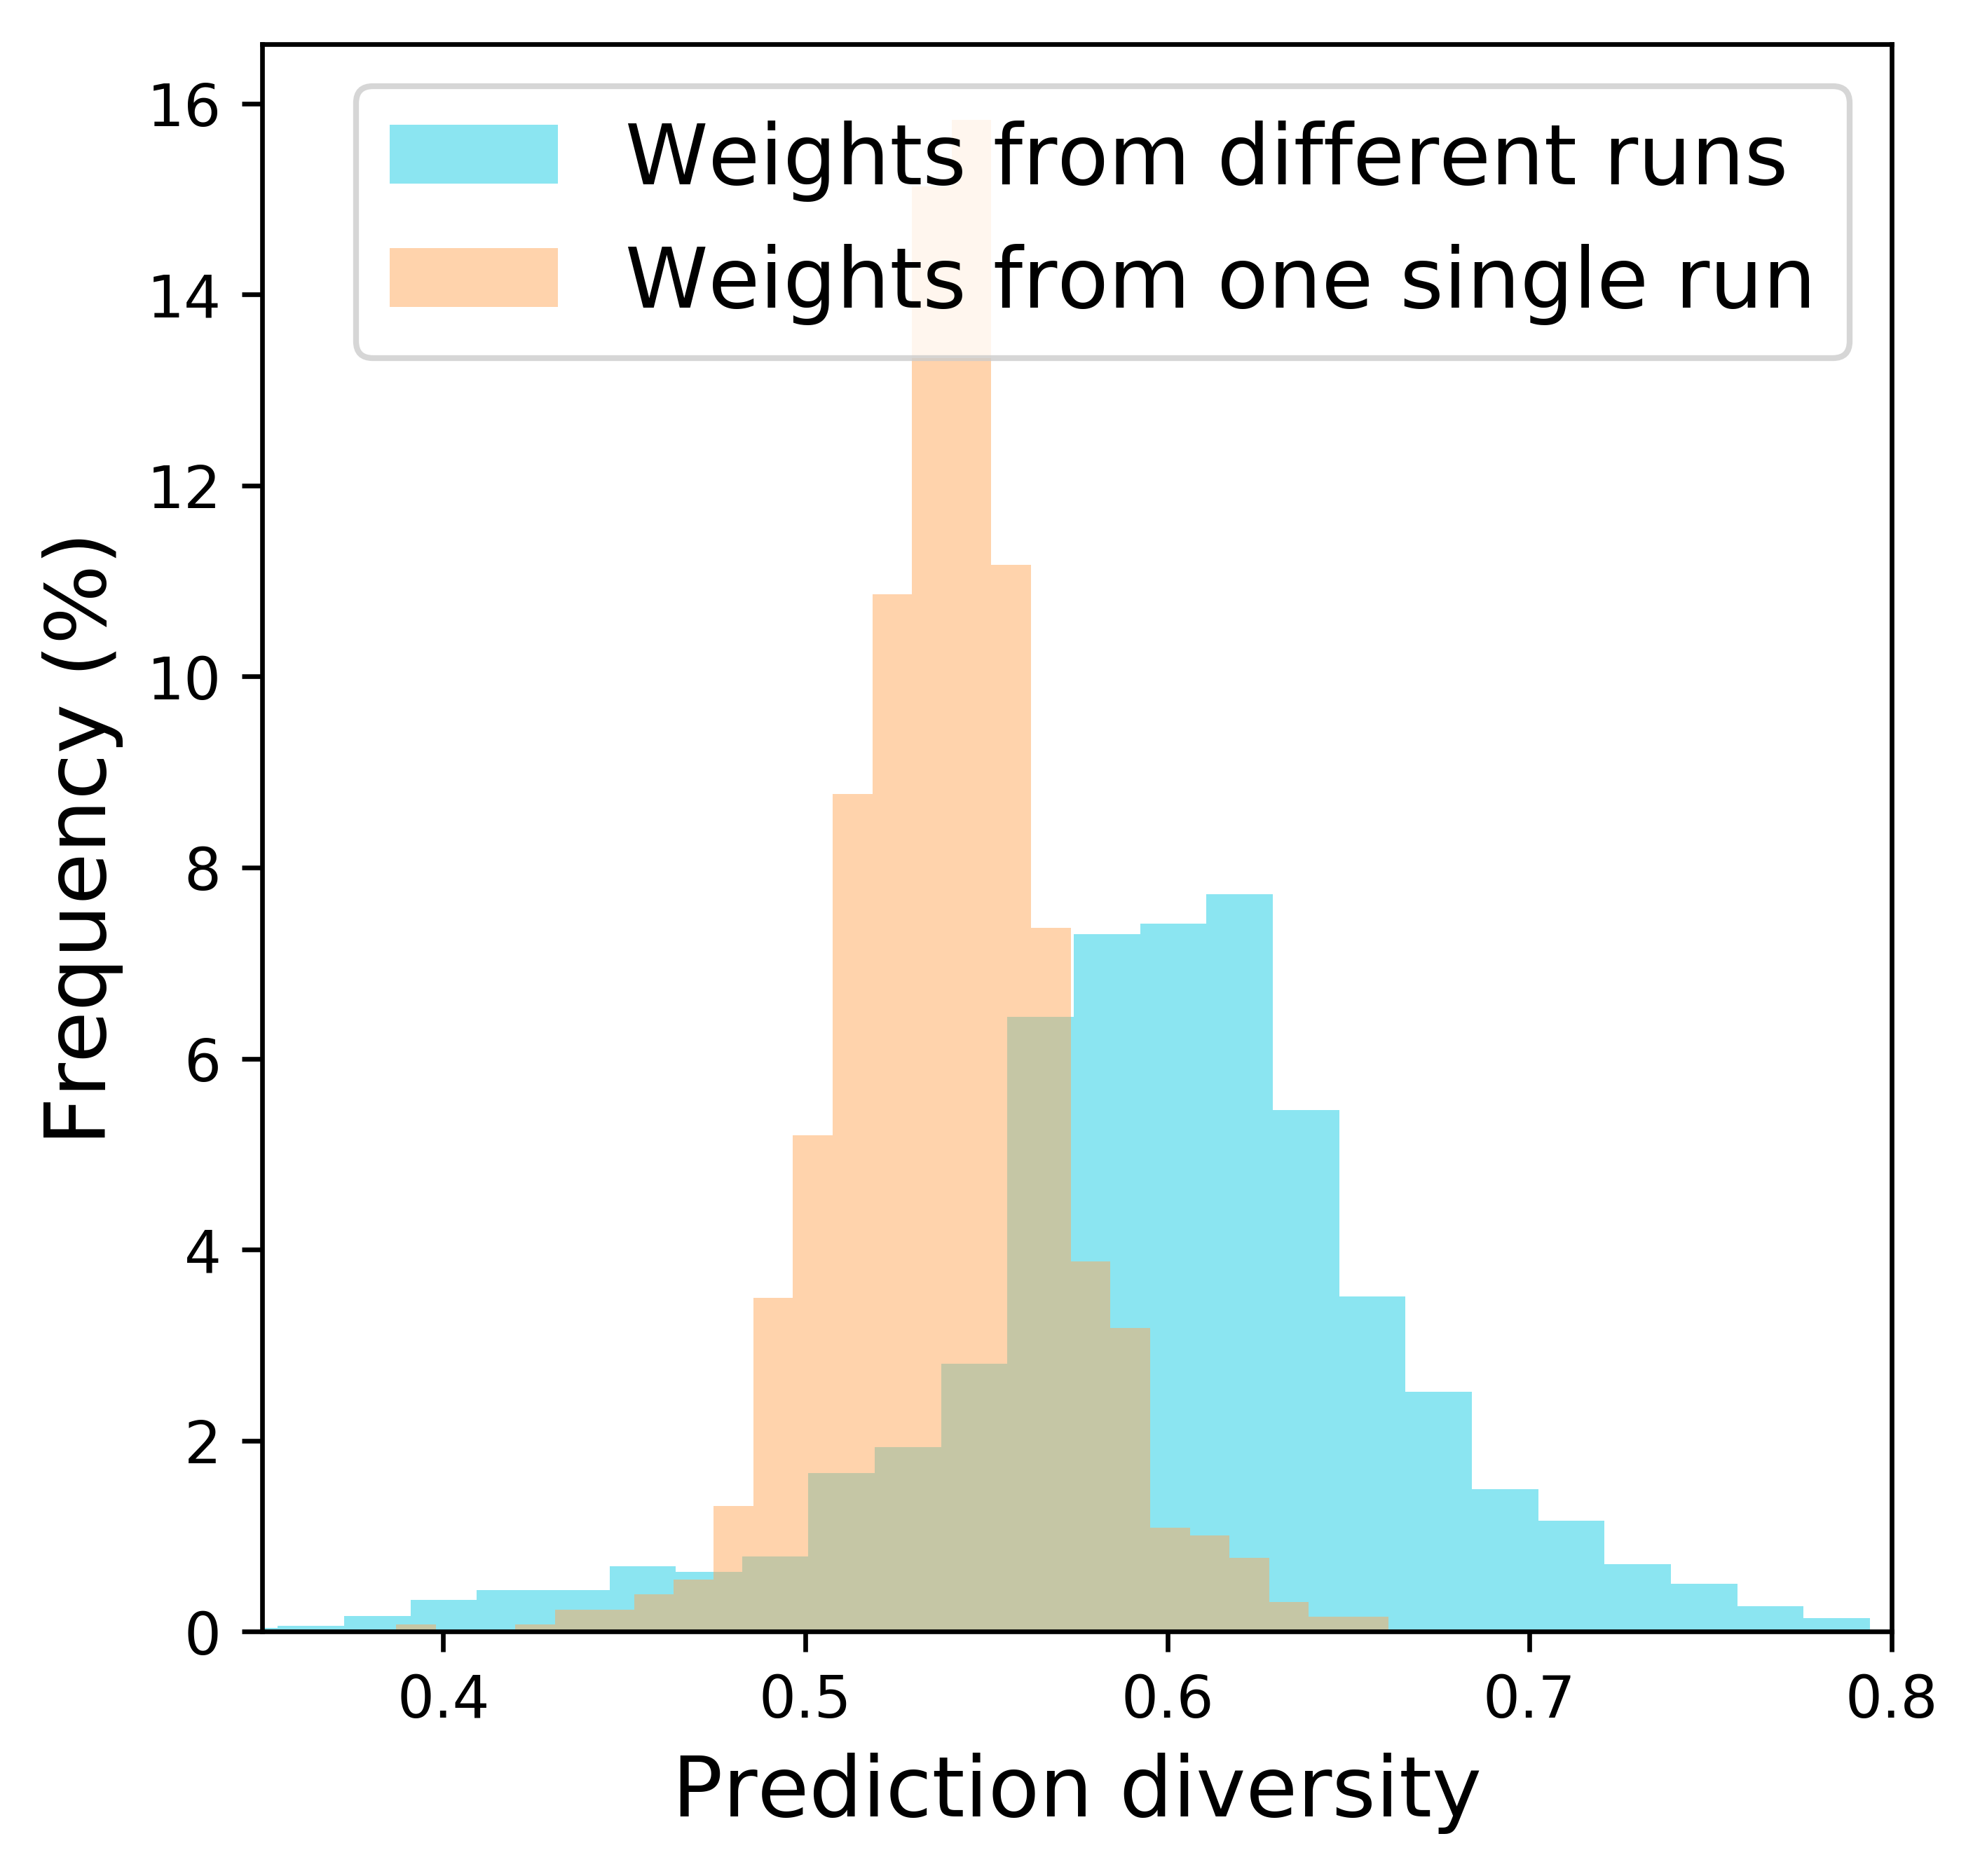
\includegraphics[width=0.9\textwidth]{pictures/files/final/home0_hist_dr.png}%
%         \caption{Diversity ($\uparrow$) across weights.}%
%         \label{fig:home0_dr_frequency}
%     \end{subfigure}%
%     \begin{subfigure}{.33\textwidth}%
%         \centering%
%         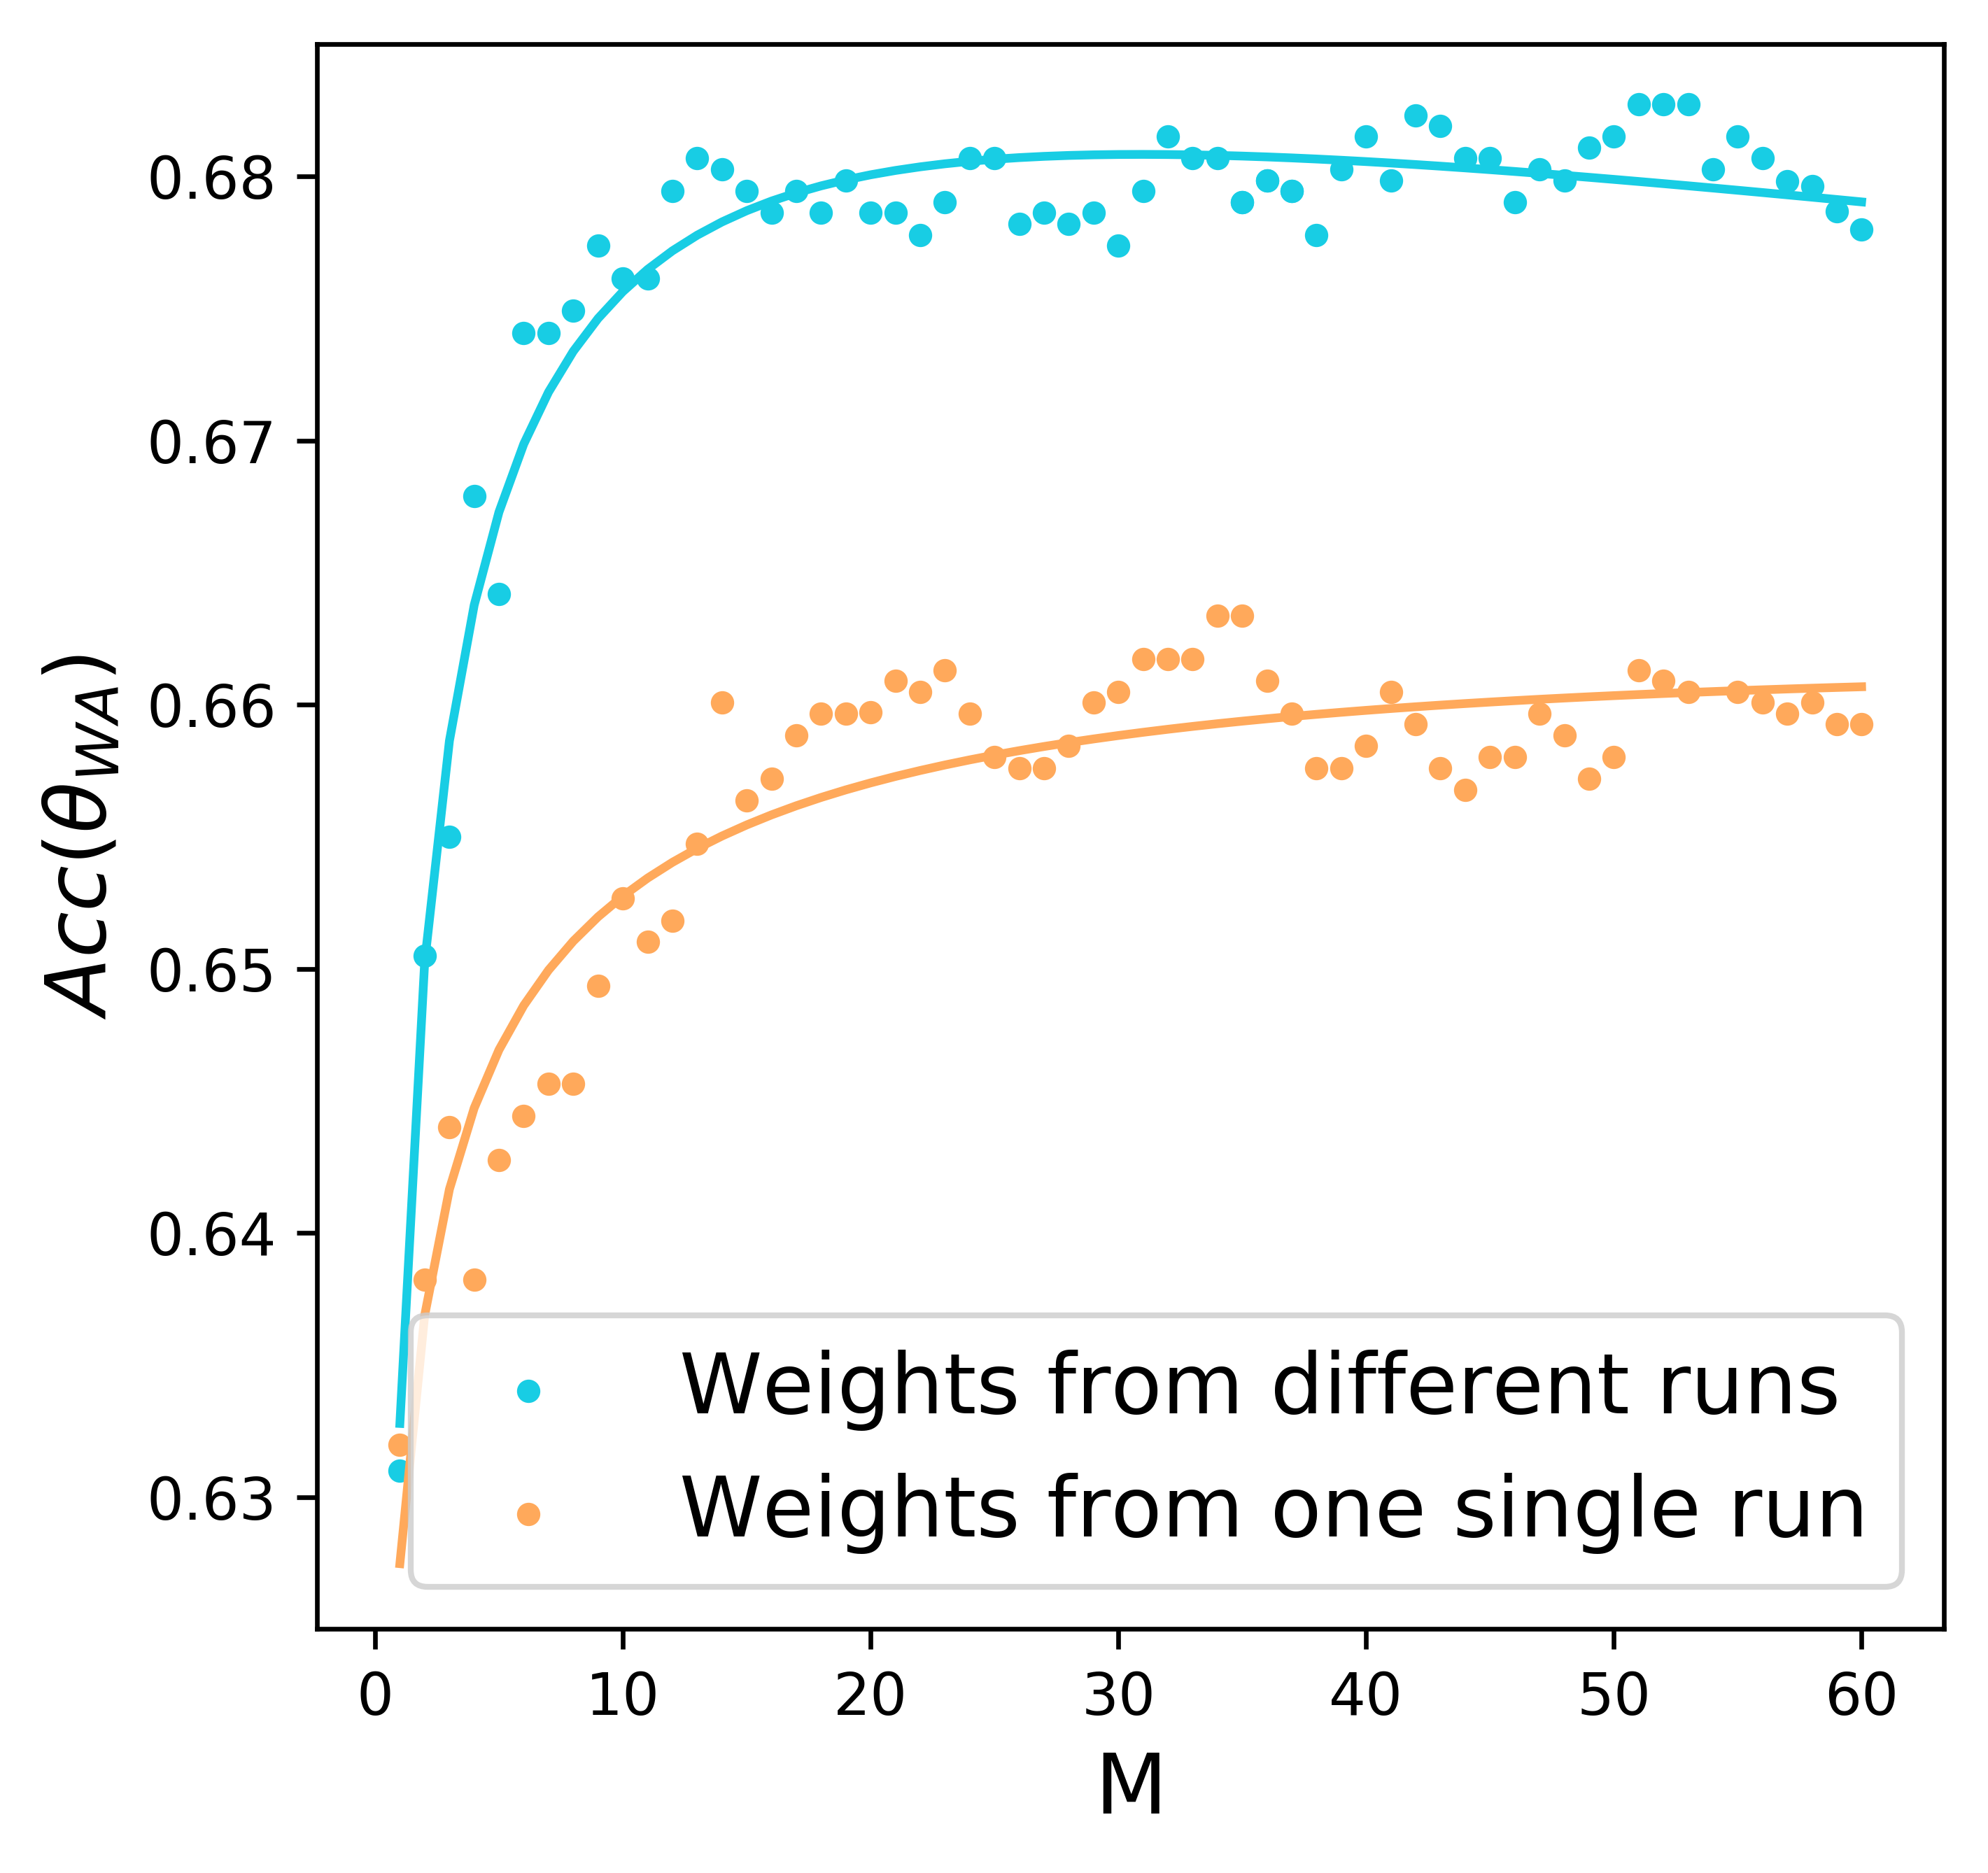
\includegraphics[width=0.9\textwidth]{pictures/files/final/home0_samediffruns_m_soup_ood.png}%
%         \caption{WA accuracy ($\uparrow$) as $M$ grows.}%
%         \label{fig:home0_m_vs_acc}%
%     \end{subfigure}%
%     \begin{subfigure}{.33\textwidth}%
%         \centering%
%         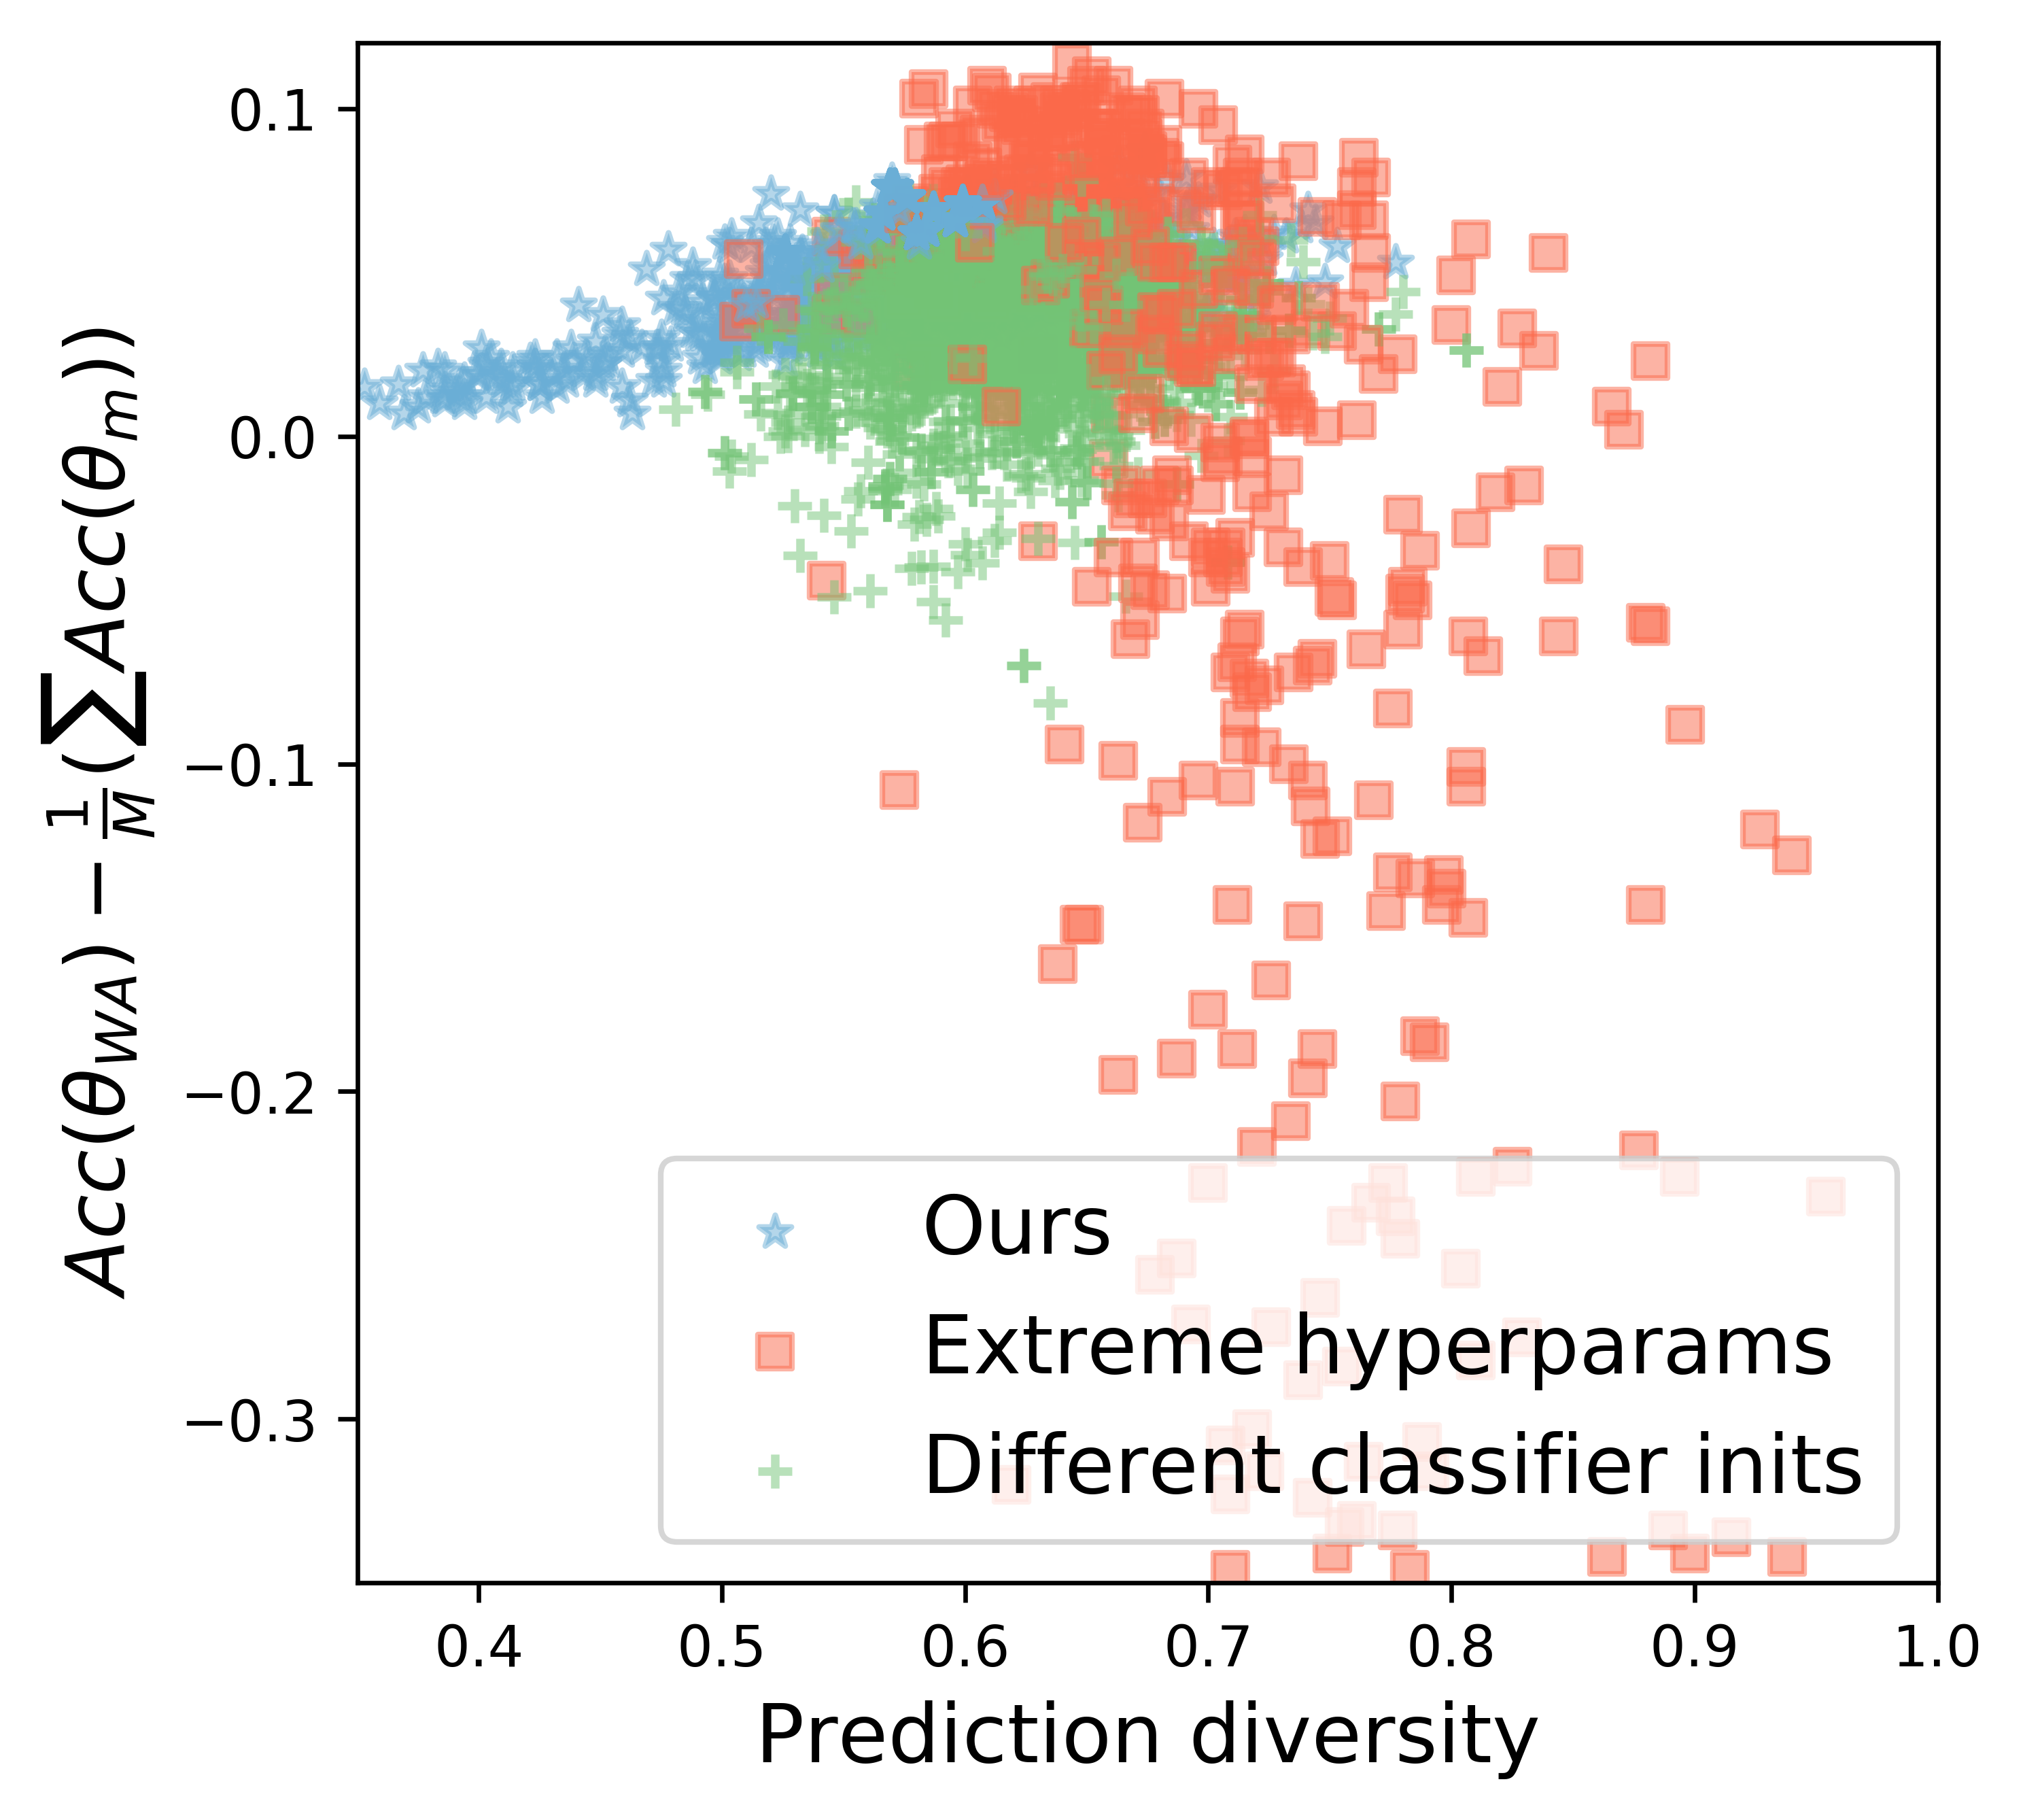
\includegraphics[width=0.9\textwidth]{pictures/files/final/home0_diffrunslargehpnosh_dr_soup-netm.png}%
%         \caption{Averaging ability.}%conditions ça ne me parait pas plus clair
%         \label{fig:home0_locality_requirement}%
%     \end{subfigure}%
%     \caption{Weights sampled from different runs are more diverse than those from a single run, and perform better after averaging, when they have close hyperparameters and shared initialization.}%
%     \label{fig:home0_dwa_vs_wa}%
%     \vspace{-1em}%
% \end{figure}%
\begin{figure}[b]
% \vspace{-0.5em}%
\begin{minipage}{.32\textwidth}%
    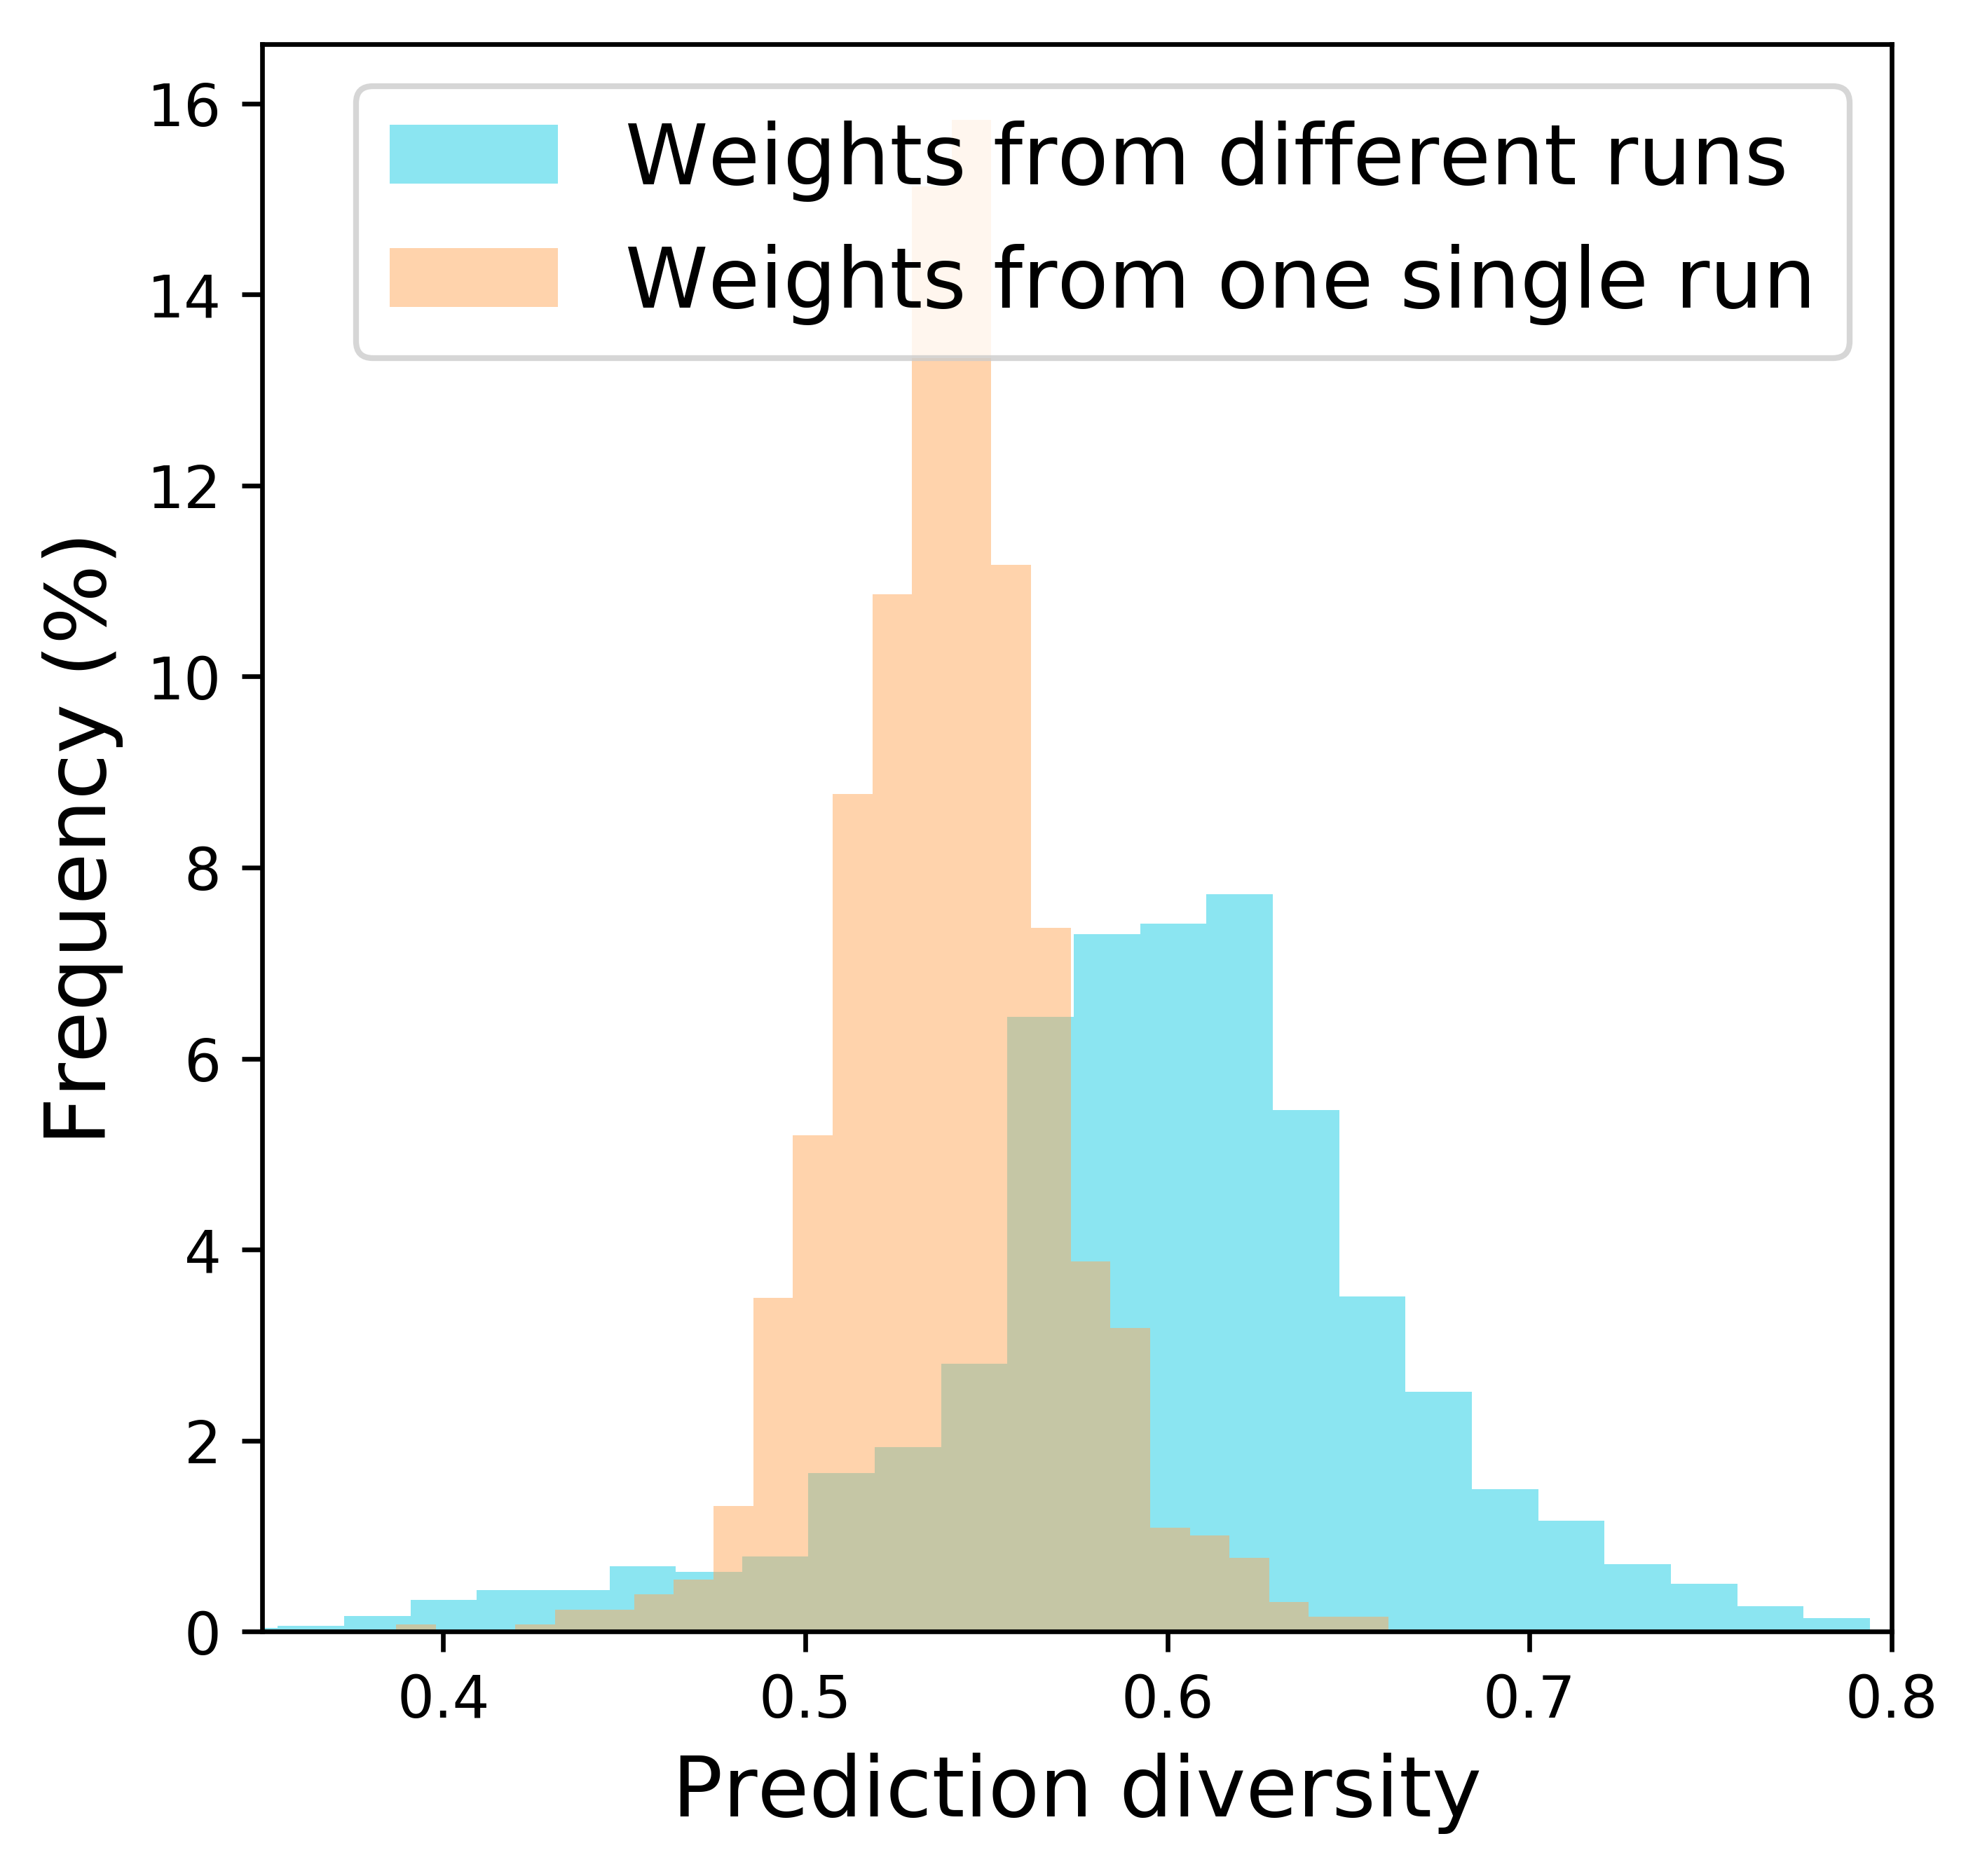
\includegraphics[width=1.0\textwidth]{pictures/files/final/home0_hist_dr.png}%
    \captionof{figure}{Frequencies of prediction diversities ($\uparrow$) \cite{aksela2003comparison} across $2$ weights obtained along a single run or from different runs.}%
    \label{fig:home0_dr_frequency}
\end{minipage}%
\hskip 1.5ex
\begin{minipage}{.32\textwidth}%
    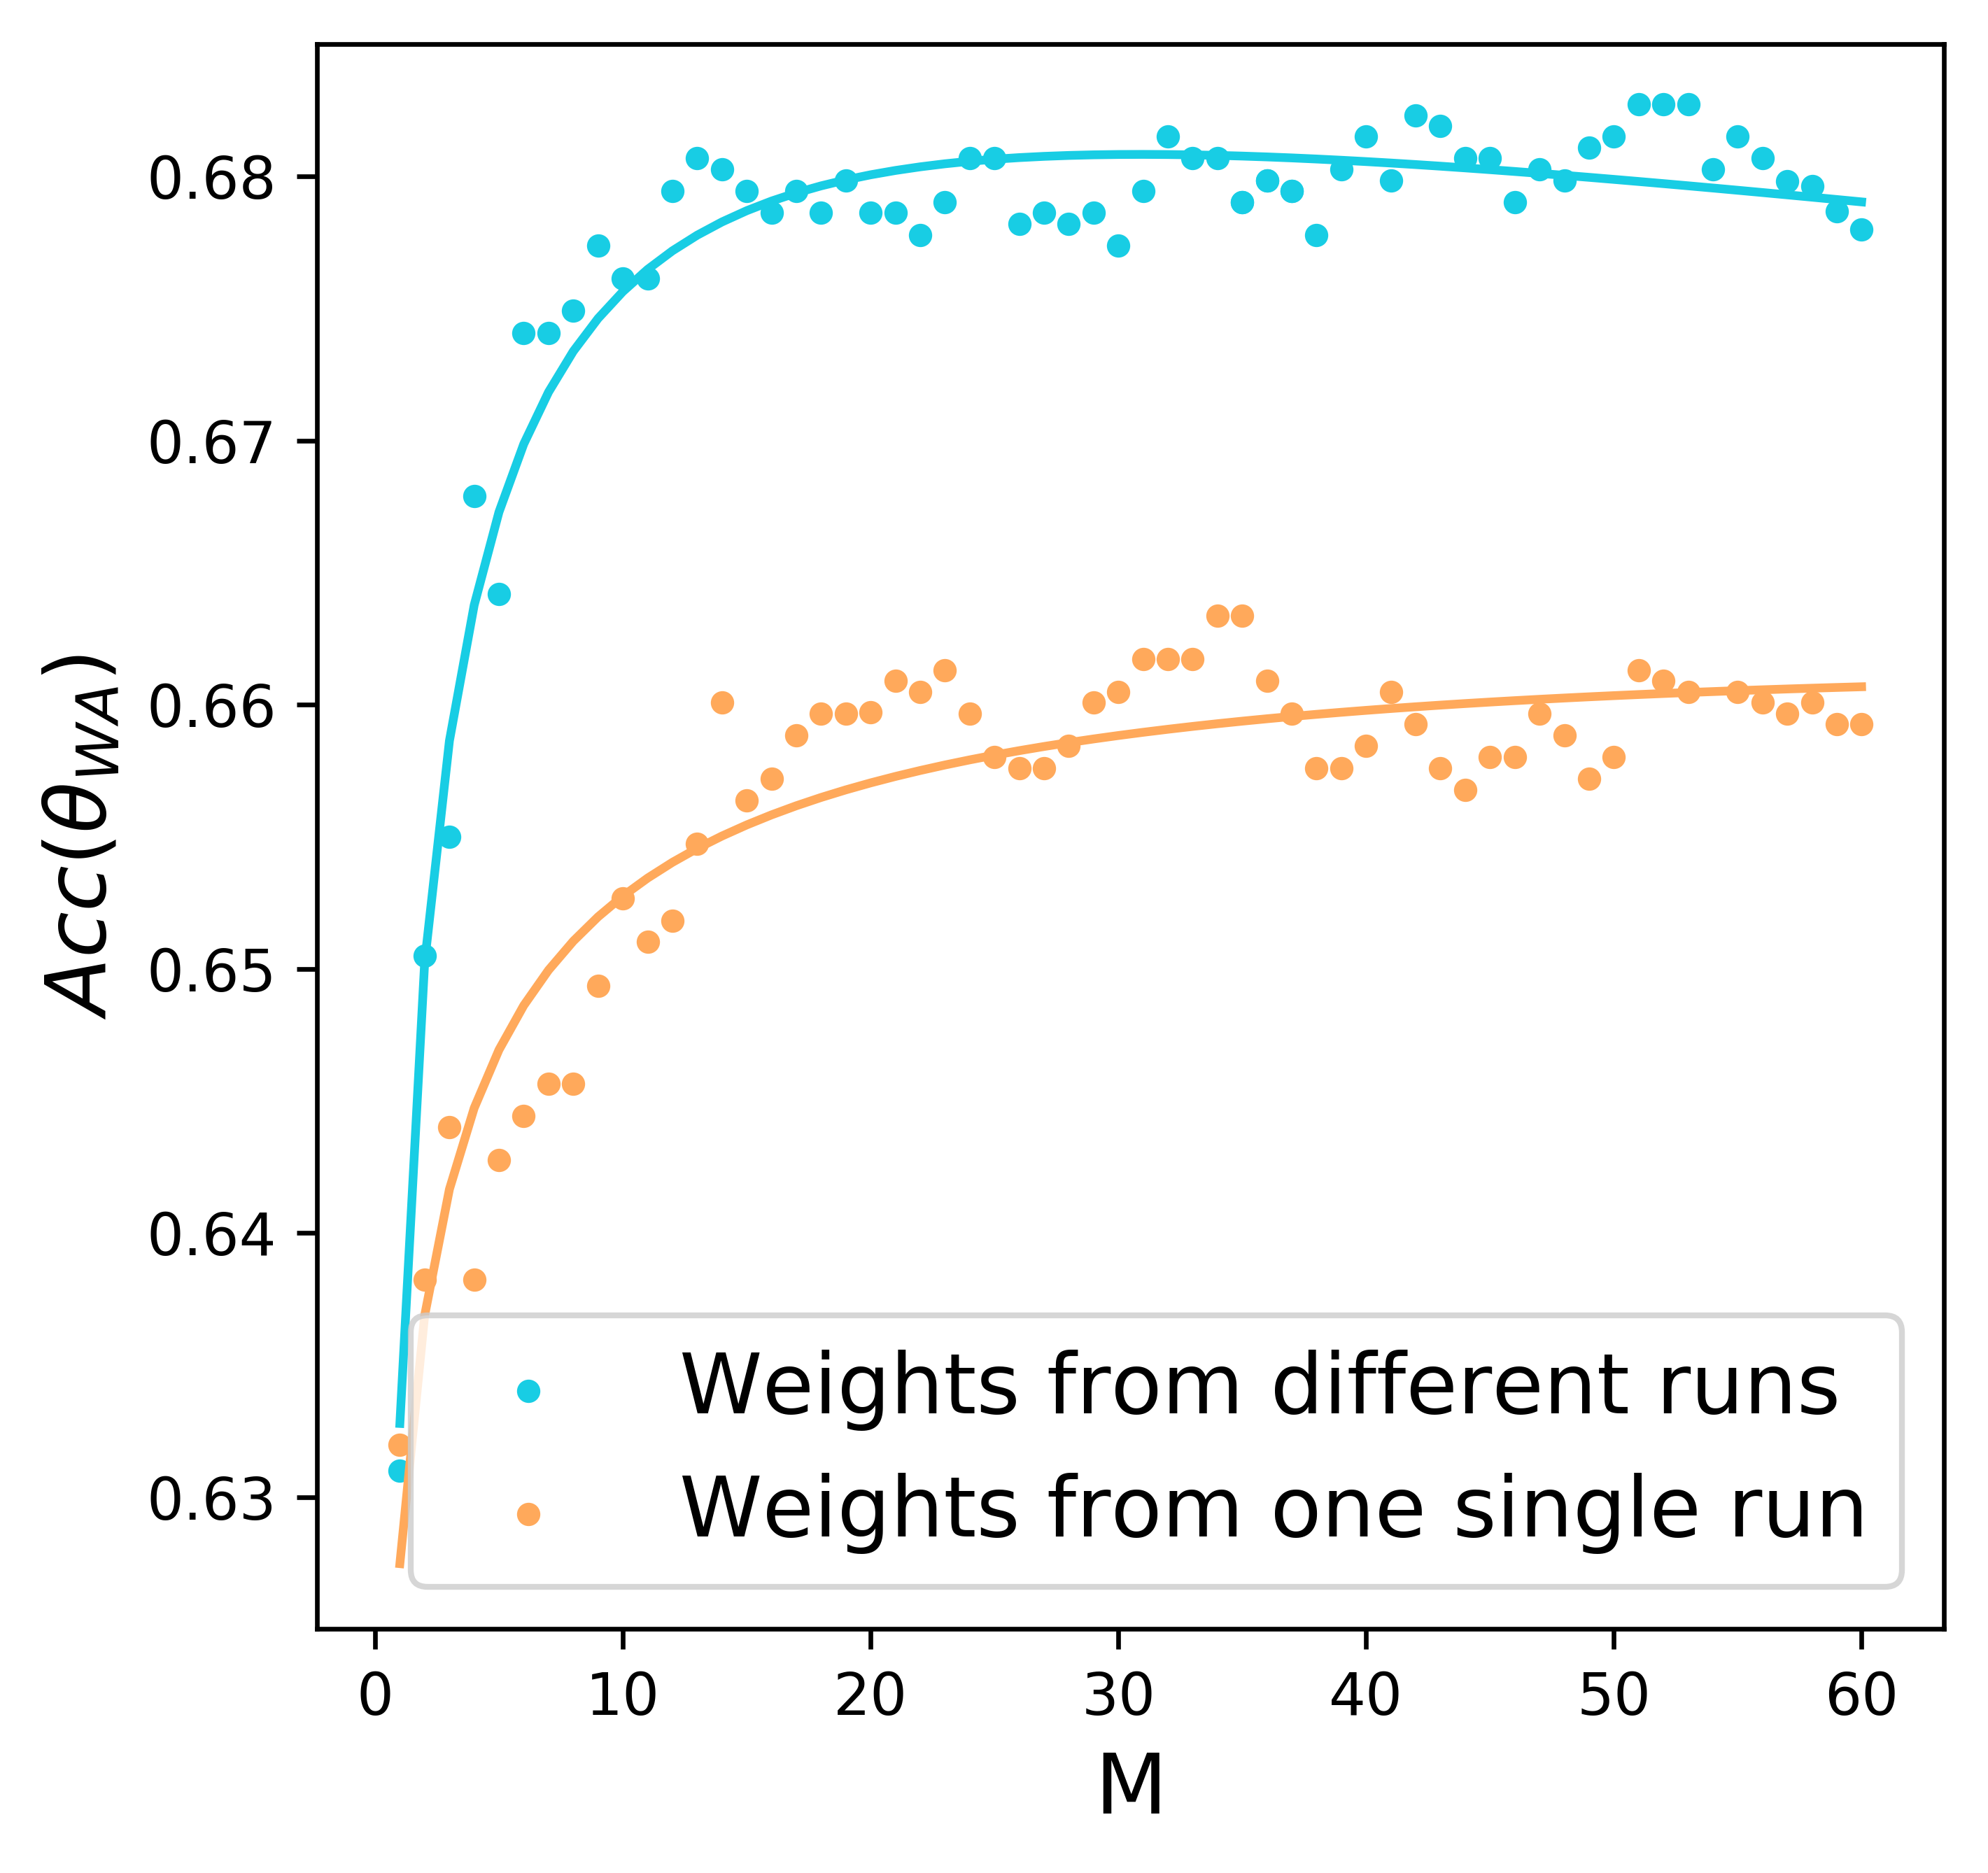
\includegraphics[width=1.0\textwidth]{pictures/files/final/home0_samediffruns_m_soup_ood.png}%
    \captionof{figure}{WA accuracy ($\uparrow$) as $M$ increases, when the $M$ weights are obtained along a single run or from different runs.}%
    \label{fig:home0_m_vs_acc}%
\end{minipage}%
\hskip 1.5ex
\begin{minipage}{.32\textwidth}%
    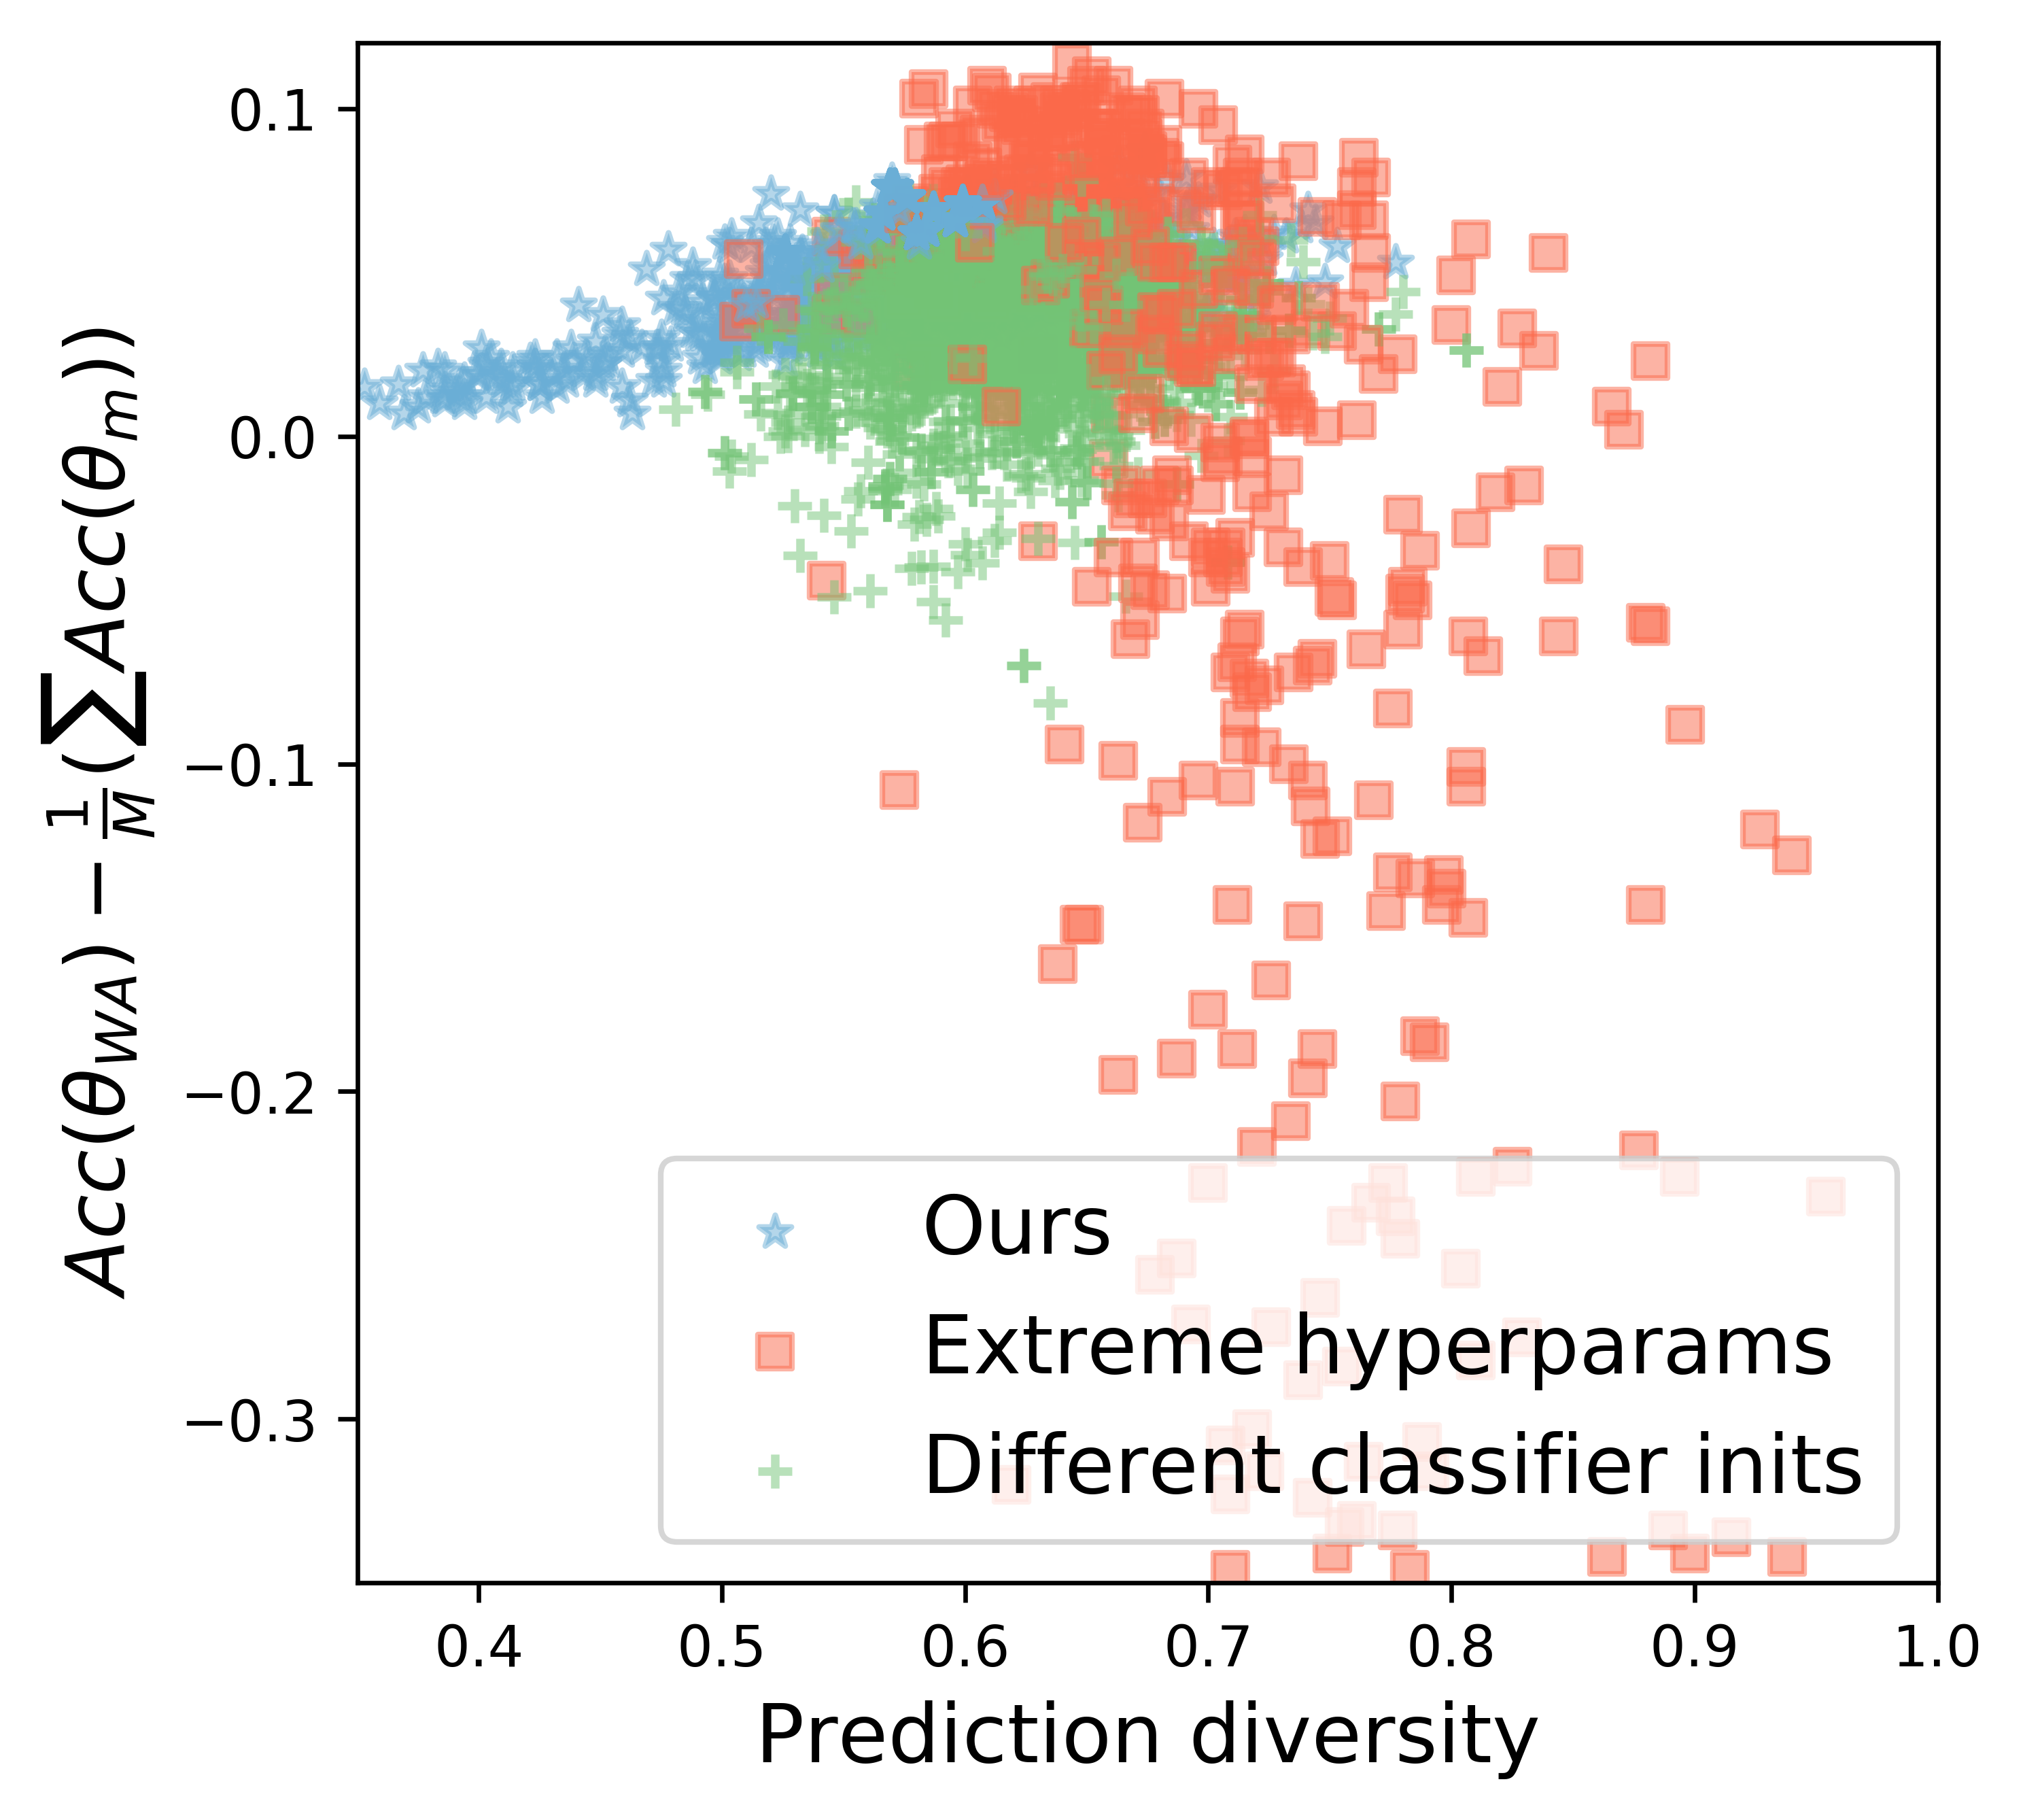
\includegraphics[width=1.0\textwidth]{pictures/files/final/home0_diffrunslargehpnosh_dr_soup-netm.png}%
    \captionof{figure}{Each dot displays the accuracy ($\uparrow$) gain of WA over its members \versus prediction diversity ($\uparrow$) for $2\leq M < 10$ models.}
    \label{fig:home0_locality_requirement}%
\end{minipage}%
\vspace{-1.em}%
\end{figure}
